\documentclass[times,10pt,twocolumn]{article} 
\usepackage[utf8]{inputenc}
\usepackage[round]{natbib}
\usepackage[spanish]{babel}
%\usepackage[verbatim]
\usepackage[titletoc,toc,title]{appendix}
\usepackage{fancyvrb}
\usepackage{hyperref} %para enlaces externos (se va a usar en los correos)

%Estos paquetes son para las tablas
\usepackage{array}
\usepackage{wrapfig}
\usepackage{multirow}
\usepackage{tabu}

%Estos paquetes son para ingluir imagenes
\usepackage{graphicx} %package to manage images
\graphicspath{ {imagenes/} }
\usepackage[rightcaption]{sidecap}

\title{\textbf{Maximización de la supervivencia de especies}}

\author{Fabián Rodríguez$^1$ y José Pablo Ureña$^2$\\
   \emph{CI-1441 Paradigmas computacionales}\\
   \emph{Escuela de Ciencias de la Computación e Informática}\\
   \emph{Facultad de Ingeniería}\\
   \emph{Universidad de Costa Rica}\\
   $^1$\emph{\href{mailto:farodriguez.49@gmail.com}{farodriguez.49@gmail.com} }, $^2$\emph{\href{mailto:jp.urenag@gmail.com}{jp.urenag@gmail.com}}$}
    \date{Diciembre de 2015}

\begin{document}

\maketitle

\begin{abstract}
%El comando \emph es para poner las cosas en italica
\emph{El presente estudio tiene como meta principal reconocer y distinguir los diferentes comportamientos asociados a un ambiente simulado de miembros, alimentación y obstáculos, donde la ''supervivencia'' y el manejo de la comunicación entre los miembros o individuos son los elementos primordiales a identificar. Basado en el impulso y estructura que permiten construir los algoritmos genéticos, esta investigación busca ser desarrollada basándose en la idea de ''evolución biologica'' que nos brindan estos algoritmos. Estudios similares aplicados a la robótica permiten ser de gran ayuda como fuente bibliográfica adicional permitiendo aclarar en gran manera la forma en como desarrollar la simulación en un ambiente de software.}\\
\end{abstract}

\noindent \textbf{Palabras clave: }supervivencia, individuos, veneno, algoritmos genéticos. 

\section{Introducción}
  Este documento describe la propuesta a un proyecto muy apegado al tema algoritmos genéticos denominado “Sobrevivencia basada en algoritmos genéticos bajo un ambiente controlado”.
Dicho proyecto tiene como idea central el buscar el desarrollo y simulación de un ambiente en el cual se encuentren individuos, desconocedores en primera instancia de su situación actual, que busquen la forma más efectiva de supervivencia en dicho medio basados principalmente en la regla de que deben alimentarse.\par
Es decir, el entorno en el que se encuentran los individuos puede verse envuelto de “comida sana” y “comida envenenada”, conforme se procede con la simulación debe buscarse la forma de mejorar la llamada variable “supervivencia”  para reducir la cantidad de individuos que mueran a causa de la comida envenenada o bien, que no logren alimentarse del todo.\par
Basados en algoritmos genéticos que buscan imitar la evolución biológica para resolver un problema, se busca implementar un entorno de simulación que tome todas estas variables y desarrolle soluciones tomando en cuenta los diferentes obstáculos que puedan enfrentar los individuos, poniendo en práctica el conocimiento computacional de paradigmas, reconociendo nuevas formas de resolver problemas y bien, desarrollando un proyecto diferente y creativo dentro de la misma área de conocimiento.\par 
En una primera instancia, se piensa implementar el proyecto por medio de sistemas multiagente, utilizando \emph{NetLogo} como plataforma para la simulación. La idea es que a cada sistema multiagente se le implemente el algoritmo evolutivo que ya se describió anteriormente.

\section{Marco Teórico}

En el campo de la inteligencia artificial existen dos enfoques básicos en la actualidad:
\begin{itemize}
    \item Enfoque simbólico.
    \item Enfoque subsimbólico.
\end{itemize}
Dentro del enfoque subsimbólico, esta el campo de la computación evolutiva y los algorítmos evolutivos, los cuales son de interés para el desarrollo de este proyecto ya que se caracterizan por crear sistemas con capacidad de aprendizaje \citep{herran1998}.\par
Los algoritmos evolutivos son procesos de búsqueda probabilística diseñados para trabajar en embientes muy grandes y que involucren estados que pueden ser representados por \emph{strings} \citep{gordbergholland1988}. \par
Es necesario que cada agente aprenda de su entorno para que, de esta manera, logre identificar posibles peligros para su supervivencia. Con respecto al aprendizaje, se puede mencionar el trabajo realizado por Dorigo y Colombeti \citep{dorigocolombetti1994} a cerca de desarrollar agentes autónomos por medio del aprendizaje. El trabajo consistió básicamente en explorar el uso de aprendizaje reforzado para "moldear" la manera en que un robot realiza una labor.Se logró conectar tanto los robots simulados como los reales a \emph{ALECSYS}, que es un sistema que implenta de forma paralela y clasificador de aprendizaje y que utiliza un algoritmo genético.\par
Desde el 2004 y hasta el 2008, un grupo de científicos del Instituto de Ciencias y Tecnologías Cognitivas, liderado por Stefano Nolfi, trabajó en un proyecto conocido como \emph{ECAgents: Embodied and Comunication Agents}. Este proyecto es de suma importancia para el trabajo actual debido a que, gracias a un breve acercamiento que tuvo uno de los miembros del proyecto con esa investigación, nace la idea de tratar de recrear algo similar al trabajo que se realizó con el proyecto \emph{ECAgents} pero en un ambiente simulado.\par
El grupo de \emph{ECAgents} \citep{nolfi2004} se encargó de implementar en unos robots, un algorítmo evolutivo que su función era lograr que los diferentes indivíduos aprendieran a comunicarse y de esta forma lograr que un robot le avisara a otro en que lugar se encontraba el alimento.

\section{Problema}
¿Cómo implementar una simulación que represente individuos que necesitan alimentarse para poder sobrevivir?\par
Lograr que los individuos que pudieron alimentarse le transmitan ese conocimiento a la siguiente generación y de esta manera, aumentar la supervivencia de la especie.\par
¿Cómo lograr que los agentes aprendan y usen el conocimiento que les han transmitido las generaciones anteriores a cerca de lo necesario para sobrevivir?
¿Será posible lograr que los agentes interactúen entre ellos y con el hambiente sin intervención humana?

\section{Objetivos y cronograma}

\subsection{Objetivo general}

Implementar un programa que mediante algoritmos evolutivos, logre que individuos pertenecientes a un ambiente simulado, puedan distinguir que elementos les proporcionan supervivencia y que elementos los eliminan del ambiente, esto a través de comunicación entre los individuos del entorno.

\subsection{Objetivos específicos}

Como parte de la implementación del programa, es de vital importancia desarrollar los siguientes aspectos dentro de la simulación, y la forma específica de comunicación entre los individuos.
\begin{itemize}
    \item \textbf{Simulación}: simular la forma en que las primeras generaciones de organismos vivos descubrieron la manera de alimentarse y transmitir esa información a las siguientes generaciones.
    \item \textbf{Sistemas multiagentes}: conocer cómo funcionan y cómo se implementan los algoritmos evolutivos en sistemas multiagente.
    \item \textbf{Comunicación evolutiva}: lograr recrear, de una manera muy básica y en un ambiente controlado, el comportamiento de seres vivos con sus necesidades más básicas (alimentarse y sobrevivir) y como le transmiten esta información a sus sucesores.
\end{itemize}

\section{Propuesta de la solución}

Para poder solucionar el problema que se planteó, se va a utilizar la herramienta \emph{NetLogo} para realizar la simulación por medio de sistemas multiagente.\par
El algoritmo genético que se quiere diseñar tiene que ser capaz de maximizar la supervivencia de la especie, con base en las variables \emph{muertes} y \emph{supervivientes}. La idea principal es que haya un método general que reciba los datos de los algorítmos genéticos que estan implementados en cada agente y que este método general haga la maximización de la variable \emph{supervivencia} junto con introducir los cambios a la siguiente generación de algorítmos.

\section{Desarrollo, prueba y validación}

\subsection{Desarrollo de la simulación}
La simulación consiste en correr el programa por una cantidad de \emph{ticks} que define el usuario. Estos \emph{ticks} representan el tiempo de vida de una generación de los agentes.\par
Durante este tiempo, se recolectan datos relevantes de la cantidad de agentes vivos y la cantidad de agentes que van muriendo.\par
Una vez finalizado el tiempo que vive una generación, se pausa la simulación, se grafican los datos y se le muestran al usuario los datos nuevos. El usuario puede entonces decidir si correr otra generación de los agentes o si finaliza la simulación.
\subsection{Desarrollo del ambiente}
El ambiente presentado para la simulación consiste en una locación en la que los agentes se pueden encontrar con ubicaciones en las que hay alimento (son 2 en el ambiente) y otras tres ubicaciones donde hay veneno.
\subsection{Desarrollo de los agentes}
Se utilizaron agentes de \emph{NetLogo} los cuales se representaron visualmente como hormigas. Cada uno de los agentes posee los siguientes atributos:
\begin{itemize}
    \item \textbf{Número de ticks vivo:} esta variable se utiliza para llevar control de cuantos ticks estuvo vivo ese agente en la generación actual.
    \item \textbf{Vida:} lleva control de la cantidad de vida restante que tiene el agente. Esta se va decrementando a medida que el agente se mueve y no encuentra alimento.
    \item \textbf{Vector de coordenadas malas:} esta es la información más importante con la que cuentan los agentes. Representa una memoria de coordenadas (\emph{x, y}) en las que el agente sabe que hay veneno. Este conocimeinto es global, esto quiere decir que todos los agentes comparten este conocimiento y ellos mismos se encargan de colaborar para que este conocimiento de posiciones peligrosas aumente.
\end{itemize}
\subsection{Desarrollo del algoritmo genético}
Al finalizar cada generación, en el conocimiento compartido de los agentes (el vector de coordenadas malas) queda almacenado todos los lugares peligrosos que encontraron los agentes de la generación que acaba de finalizar.\par
Gracias a lo anterior, la siguiente generación de agentes ya va a contar con más información de lugares en los que hay veneno y por lo tanto, que tienen que evitar.\par
\subsection{Paso del conocimiento}
La estructura de comunicación elegida para los agentes es la de memoria compartida (o pizarra) y esa memoria es representada por el vector de coordenadas malas.\par
Cada vez que un agente se encuentra con un agente muerto, este se encarga de marcar esa posición como peligrosa y agregarla a la memoria que comparten todos los agentes.
\subsection{Problemas encontrados}
\label{subsec:problemas_encontrados}
\begin{itemize}
    \item \textbf{Manejo de listas en NetLogo}\par 
    El manejo de listas en NetLogo supuso un problema al inicio del desarrollo debido a que el lenguaje en sí no presenta muchas facilidades para poder hacer uso de estas estructuras de datos.\par
    Debido a esto, se tuvo que reformular la solución que se había planteado al inicio. Originalmente cada agente iba a contar con su vector de coordenadas buenas y malas propio, que posteriormente se iba a compartir con los agentes que se topara. Por problemas que se presentaron al intentar implementar esta manera de compartir la información, fue que se optó por utilizar (en lugar de la memoria propia del agente) la pizarra donde los agentes comparten la información. 
\end{itemize}

\section{Experimentación y análisis}
El experimento consistió en correr la simulación inicialmente sin la implementación del algoritmo genético y posteriormente con el algoritmo implementado.\par
Lo anterior se desarrolló de esta manera para poder hacer una comparación que evidenciara la diferencia (de existir alguna) entre la supervivencia de los agentes que no tenían conocimiento alguno de las ubicaciones con veneno vs. los agentes que si tenían esta información.\par
Para la recolección de los datos del experimento, se corrió la simulación treinta veces, con un tiempo de simulación de 1500 ticks y sin haber implementado el algoritmo genético. De esta manera, los agentes simplemente deambulaban por el entorno sin conocer nada a cerca de él y una vez que se encontraban con veneno los individuos morían. El el Cuadro \ref{table:sinalggen} se puede observar los datos obtenidos corriendo la simulación de esta manera y en la Figura \ref{fig:sinalg} se exponen todos los datos obtenidos. Es importante recalcar que en la Figura \ref{fig:sinalg} se ve como en todos los casos, la cantidad de agentes muertos es superior a la cantidad de agentes vivos.\par
Una vez obtenidos estos datos, se corrió la simulación otras treinta veces, con 1500 ticks de tiempo cada corrida pero esta vez con el algorítmo genético implementado. Los datos obtenidos se pueden observar en el Cuadro \ref{table:conalggen}. Al correr la simulación de esta manera, se puede observar como los agentes, paulatinamente, empiezan a evitar las zonas en las que otros agentes murieron. Esto hace que la supervivencia de los agentes aumente considerablemente, algo que se puede verificar en los datos que se obtuvieron.\par
Es interesante observar en la Figura \ref{fig:conalg} como se ve que al implementar al algorítmo genético, se presenta una tendencia a que cada generación aumente la cantidad de agentes que permanecieron vivos y dismunuya la cantidad de muertes.\par


    \begin{table}[h!]
    \centering
    \caption{Media sin el algoritmo genético}
    \hfill\break
    \begin{tabular}{c c}
    Estado & Media (cantidad de agentes) \\ [0.5ex]
    \hline
    Vivos & 128\\
    Muertos & 171\\
    \end{tabular}
    \label{table:sinalggen}
    \end{table}
    
    \begin{figure}[h!]
        \centering
            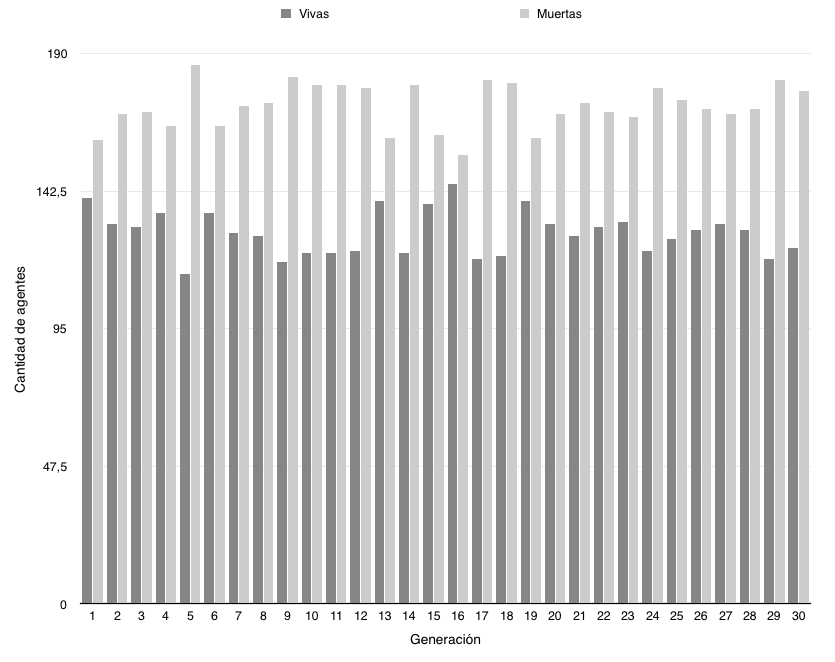
\includegraphics[width=0.50\textwidth]{sinalg}
            \caption{Datos obtenidos sin el algoritmo genético}
            \label{fig:sinalg}
    \end{figure}
    
    
    \begin{table}[h!]
    \centering
    \caption{Media con el algoritmo genético}
    \hfill\break
    \begin{tabular}{c c}
    Estado & Media (cantidad de agentes) \\ [0.5ex]
    \hline
    Vivos & 227\\
    Muertos & 73\\
    \end{tabular}
    \label{table:conalggen}
    \end{table}
    
    \begin{figure}[h!]
        \centering
            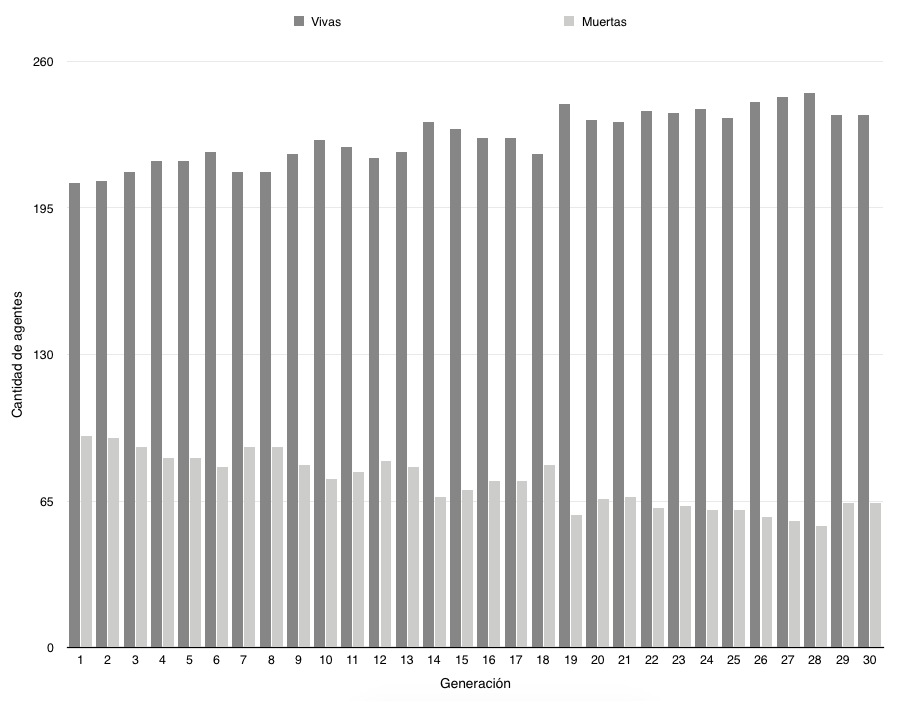
\includegraphics[width=0.50\textwidth]{conalg}
            \caption{Datos obtenidos con el algoritmo genético}
            \label{fig:conalg}
    \end{figure}

Después de haber obtenido toda esta información, se pudo proceder a comparar los datos de ambos experimentos para así determinar, si efectivamente se había obtenido una mejora en la supervivencia de los agentes al implementar el algoritmo genético.\par
Al observar el Cuadro \ref{table:sinalggen} y el Cuadro \ref{table:conalggen} se puede determinar que efectivamente se logró una mejora sustancial en la media de la cantidad de agentes que sobrevivieron en las treinta corridas de la simulación. Más visualmente, se puede ver la superioridad en la supervivencia de las especies en la Figura \ref{fig:comparacion} donde se muestra lado a lado las medias de los supervivientes y muertes obtenidas al haber corrido la simulación con y sin el algoritmo genético.

    \begin{figure}[h!]
        \centering
            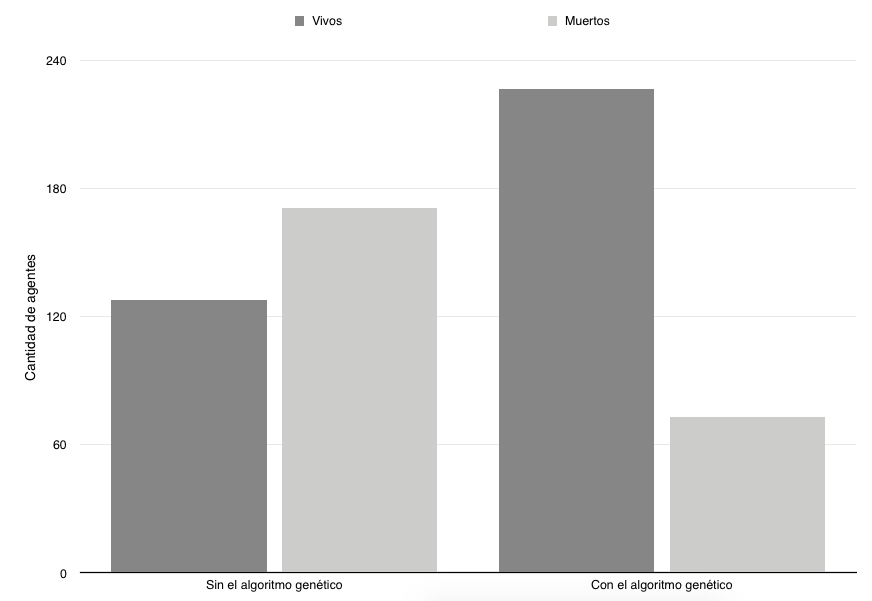
\includegraphics[width=0.50\textwidth]{comparacion}
            \caption{Comparación de las medias del experimento}
            \label{fig:comparacion}
    \end{figure}

Gracias a la información arrojada por el experimento, se puede concluir que se logró satisfacer el objetivo principal de la investigación. Efectivamente, se logró implementar un programa que hiciera que individuos en un ambiente controlado lograran diferencias entre alimento y veneno. En los datos que se recopilaron se puede apreciar que gracias a esto, la población logró aumentar considerablemente su supervivencia.

\section{Problemas abiertos y problemas futuros}

\subsection{Manejo de memoria propia para cada agente}
Se propone implementar el programa pero de manera que el manejo del conocimiento sea distinto.\par
Sería interesante observar el comportamiento de los agentes haciendo el cambio de que en vez de que utilicen memoria compartida, cada agente tenga su propio vector de coordenadas malas y que este conocimiento se lo transmitan a los demás individuos al toparse con ellos durante la simulación.\par
Como se explicó en la subsección \ref{subsec:problemas_encontrados}, originalmente se planteó la solución sin utilizar memoria compartida pero por los inconvenientes presentados durante el desarrollo del sistema, se optó por esta manera para compartir la información.\par
Es por esto que queda abierto a los interesados implementar la solución que aquí se propuso utilizando esta forma de manejar el conocimiento.

\subsection{Optimización del tiempo de la simulación}
El usuario podrá notar que al ejecutar la simulación utilizando el algorítmo genético, el tiempo que dura en correr aumenta significativamente.\par
Se propone a los interesados que se determine alguna manera en que se logre mejorar el tiempo de respuesta de la simulación. Se piensa que el aumento en el tiempo se debe a la gran cantidad de agentes que están tratando de leer y escribir en el recurso compartido (el vector de coordenadas). Lo anterior ocaciona que NetLogo tenga que hacer una sincronización entre todos los agentes y esto se cree que es lo que repercute en el tiempo de la simulación.

\section{Anexos}
Todo el código del proyecto se puede consultar y descargar del siguiente \href{https://github.com/fabo49/SupervivenciaDeEspecies}{repositorio en GitHub.} En él se encuentra tanto el código del proyecto como los resultados obtenidos y el código \LaTeX ~de este artículo.
\bibliographystyle{plainnat}
\bibliography{bibliografia}

\end{document}